\section{Comparisons for the complete return}\label{sec:return-comparisons}\label{sec:counting}

Three scalar comparisons give the upper bound on the complete actual
returning interval of one fixed field. They compare a simple-contact
passage with its complement, control a derivative ratio through slow-root
collision, and compose two endpoint passages with their signed connector.
The physical domains and estimates needed to apply them are proved in
Sections~\ref{sec:positive-constant} and~\ref{sec:two-endpoints}, and
Appendix~\ref{sec:simple-contact}.

\subsection{A simple-contact passage and its complement}
\label{subsec:simple-comparison-core}
For a simple contact with positive preceding slow speed, the bound two
comes from a derivative comparison of the local passage with its
complement. Near the central saddle-node, let $W$ be the scalar
speed in the orbital product coordinates. The passage from the fixed
incoming section $w=w_0>0$ to $s=s_+$ is
$D(s)=w_0\exp(-\int_s^{s_+}dt/W(t))$; write its increasing
complement as $H(a)$. On a subinterval containing every return zero,
the finite-passage condition and complement estimates give $W(H)>0$ and
\[
 \frac{d}{da}\log\frac{D(H(a))}{a}
   =\frac{Z(a)}{aW(H(a))},\qquad
 Z=aH'-W(H),\qquad
 Z'=H'\left(1-W_s(H)+a\frac{H''}{H'}\right)>0.
\]
The logarithmic displacement therefore has at most one stationary
point, a strict minimum. In the saddle ranges, the corresponding
comparison makes every zero of $(D\circ H)'-1$ a strict downward
crossing. For the weak saddle this follows directly from the exact
power $D(s)=\xi_0(s/\omega_0)^r$, $0<r\leq r_0<1$: at $(D\circ H)'=1$,
\[
 (D\circ H)''=\frac{r-1}{rD(H)}+\frac{H''}{H'}<0,
\]
because the complete complement satisfies $r|H''/H'|=o(1)$.
The finite-ratio Dulac estimates give the same conclusion, including
ratios approaching one. In each case a tangent zero is exactly
quadratic and exhausts the local count two.

In the weak-saddle range, early departures form the upper interval
of the physical source, and their displacement is strictly decreasing.
The late interval has the single-maximum property just proved.
After two simple late zeros, or one quadratic late zero, its displacement
is negative up to the finite threshold; continuity and strict decrease
then exclude a threshold or early zero. Otherwise each interval
contributes at most one simple zero. This gives total multiplicity two
on the whole return domain. The local conjugacy is used only where its
outgoing continuation and inverse are both defined; all late outputs
lie in that common image. Appendix~\ref{sec:simple-contact} proves
these domain statements and the derivative estimates above.

\subsection{A weighted derivative ratio through slow-root collision}
\label{subsec:collision-comparison-core}
Let $q_0$ be the scaled incoming height and $\beta$ the fixed-field
separator height on that cut. On the no-root side, $\beta$ is the trace
of the physical outgoing tail; on the root side it is the trace of the
selected incoming stable or parabolic separator. In both cases the actual
returning domain has source distance $s=q_0-\beta>0$.
The incoming reference $q_c(0)$ controls distortion through
$w_\beta=\beta-q_c(0)$; $\beta$ determines the returning boundary.
Section~\ref{sec:positive-constant} constructs these objects and proves
the incoming and outgoing bounds used in the following comparison.

\begin{lemma}
\label{lem:pc-ratio}
Suppose that on an actual returning interval
$s=q_0-\beta>0$, where $\beta$ is independent of $u_{\rm up}$,
$w_\beta=\beta-q_c(0)>0$, and $w_0=s+w_\beta\le C_0$.
Write $M(s)=\partial_s T_+>0$. Assume that, for some $\delta>0$,
\begin{equation}
\label{eq:pc-outgoing-conditions}
 sM(s)\le\varepsilon^2\delta\quad(s\in I),\qquad
 -s(\log M)_s\ge c_M>0\quad(s\in I\cap(0,s_0]),
\end{equation}
where $I$ is the actual returning interval and $s_0,c_M>0$ are fixed.
Assume also that the incoming transition has
\begin{equation}
\label{eq:pc-entry-slope-for-ratio}
 \begin{aligned}
 s_{u_{\rm up}}&=-\varepsilon^{-2}\lambda(s+w_\beta),\qquad
 0<c_\lambda\le\lambda\le C_\lambda,\quad 0<c_j\le j\le C_j,\\
 |(\log\lambda)_{u_{\rm up}}|&\le L_\lambda\varepsilon^{-2},\qquad
 |(\log j)_{u_{\rm up}}|\le L_j.
 \end{aligned}
\end{equation}
on $I$, where all bounds are fixed. These are the incoming and
short-transition estimates from Lemma~\ref{lem:pc-entry} and
\eqref{eq:short-map}. Fix $0<\varepsilon\le\bar\varepsilon$ and put
$K=L_\lambda+C_\lambda+\bar\varepsilon^2L_j$. Require
\begin{equation}\label{eq:pc-ratio-smallness}
 4C_\lambda\delta\le c_j,\qquad
 \delta\le\frac{c_Mc_j}{4K}.
\end{equation}
If the curvature bound is only available for $s\le s_0$, require also
\begin{equation}\label{eq:pc-ratio-localization}
 \frac{4C_\lambda\delta}{c_j}w_\beta<s_0.
\end{equation}
This last condition may be replaced by
$2C_\lambda\delta C_0/c_j<s_0$; it is unnecessary when the curvature
bound holds throughout $I$. Then the isolated return zeros of $T_+-T_-$
have total actual multiplicity at most two.
\end{lemma}

\begin{proof}
Write $u=u_{\rm up}$ and let $R=M|s_u|/j$. The size and incoming bounds give
\[
 R\le\frac{C_\lambda\delta}{c_j}\frac{s+w_\beta}{s}.
\]
Where $R\ge1/2$, the first condition in \eqref{eq:pc-ratio-smallness}
therefore gives
\begin{equation}\label{eq:pc-ratio-source-bound}
 s\le\frac{2C_\lambda\delta}{c_j-2C_\lambda\delta}w_\beta
   \le\frac{4C_\lambda\delta}{c_j}w_\beta.
\end{equation}
Before absorption the same inequality gives
$s\le2C_\lambda\delta(s+w_\beta)/c_j\le2C_\lambda\delta C_0/c_j$.
Thus either cutoff above places these points in the curvature range.
Its logarithmic derivative is
\[
 (\log R)_u=(\log M)_s s_u+
                 (\log\lambda)_u-\varepsilon^{-2}\lambda-(\log j)_u.
\]
At these points $M|s_u|\ge j/2$, so
$|s_u|/s\ge c_j/(2\varepsilon^2\delta)$. The second condition in
\eqref{eq:pc-ratio-smallness} now yields
\[
 (\log R)_u\ge\frac1{\varepsilon^2}
       \left(\frac{c_Mc_j}{2\delta}-K\right)
       \ge\frac{c_Mc_j}{4\varepsilon^2\delta}>0.
\]
Thus $R_{u_{\rm up}}>0$ wherever $R\ge1/2$.
It crosses one at most once, strictly upward.
Since $(T_+-T_-)_{u_{\rm up}}=j(1-R)$, there is at most one stationary
point, a strict maximum. At a stationary return zero,
$(T_+-T_-)_{u_{\rm up}u_{\rm up}}=-jR_{u_{\rm up}}<0$.
Such a zero is quadratic and cannot coexist with another return zero.
Otherwise there are at most two simple zeros. Section~\ref{sec:return-framework}
transfers these orders to actual minimal-return multiplicity.
\end{proof}

In the collision product coordinate, $\eta_0>0$ is the fixed normal
exit height. Write $A$ and $B$ for the normal amplitudes at the left
and right bases. Lemma~\ref{lem:pc-collision-localization} gives an
open physical returning interval $I_{\rm ret}$ on which $0<A<\eta_0$;
every counted cycle has $A<\eta_0/2$.
On the no-root side $B=m_bA$, where $m_b>1$ is the normal expansion
through the strip, without a uniform upper bound. The through and
fibre-exit pieces are the intersections of the actual source with
$0<A<\eta_0/m_b$ and $\eta_0/m_b<A<\eta_0$, respectively.
They are ordered by increasing source distance $s$, opposite to
$u_{\rm up}$, and have at most one finite common boundary.
On the root side only the fibre-exit piece occurs.
Figure~\ref{fig:collision-passages} depicts this partition.
Lemma~\ref{lem:pc-source-partition} includes empty pieces and the finite boundary.

% Schematic product-coordinate passages, not numerical DF1b trajectories.
% Representative curves solve d eta/d theta = .65 eta in drawing units.
% The half-amplitude tick localizes counted zeros; it is not a passage event.
% Native size: approximately 108 mm wide, with 10 pt labels.
\begin{figure}[H]
\centering
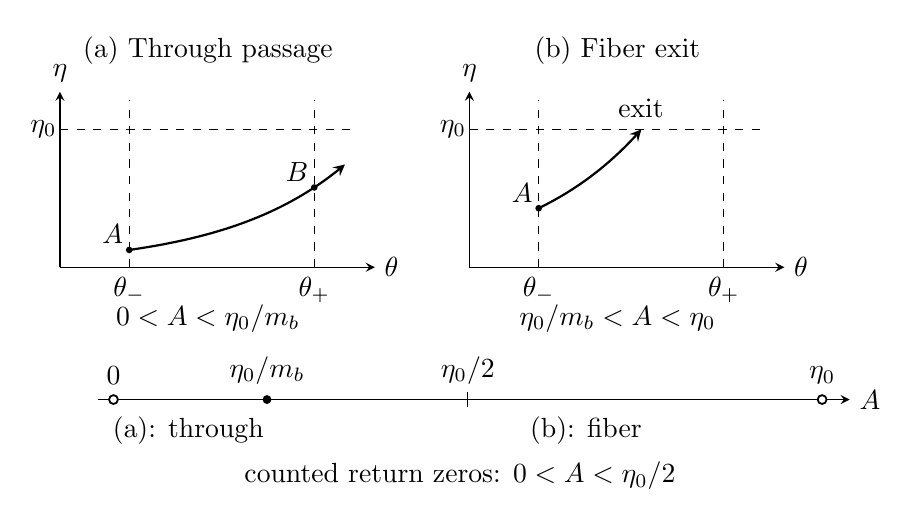
\begin{tikzpicture}[x=10mm,y=10mm,>=stealth,
  every node/.style={font=\fontsize{10}{12}\selectfont},
  axes/.style={->,line width=.45pt},
  section/.style={dashed,line width=.5pt},
  orbit/.style={->,line width=.8pt}]
  \foreach \shift/\panel/\heading in
    {0/a/Through passage,5.2/b/Fiber exit} {
    \begin{scope}[xshift=\shift cm]
      \node at (2,2.75) {(\panel) \heading};
      \draw[axes] (.12,0)--(4.12,0) node[right] {$\theta$};
      \draw[axes] (.12,0)--(.12,2.23) node[above] {$\eta$};
      \draw[section] (1,0)--(1,2.12);
      \draw[section] (3.35,0)--(3.35,2.12);
      \draw[section] (.12,1.75)--(3.83,1.75);
      \node[below] at (1,0) {$\theta_-$};
      \node[below] at (3.35,0) {$\theta_+$};
      \node[left,inner sep=1pt] at (.12,1.75) {$\eta_0$};
    \end{scope}
  }
  \begin{scope}
    \draw[orbit,domain=1:3.74,samples=45,smooth]
      plot (\x,{.22*exp(.65*(\x-1))});
    \fill (1,.22) circle (1.2pt);
    \fill (3.35,{.22*exp(.65*2.35)}) circle (1.2pt);
    \node[above left,inner sep=2pt] at (1,.22) {$A$};
    \node[above left,inner sep=2pt] at (3.35,{.22*exp(.65*2.35)}) {$B$};
    \node at (2,-.65) {$0<A<\eta_0/m_b$};
  \end{scope}
  \begin{scope}[xshift=5.2cm]
    \draw[orbit,domain=1:2.303535169826467,samples=35,smooth]
      plot (\x,{.75*exp(.65*(\x-1))});
    \fill (1,.75) circle (1.2pt);
    \node[above left,inner sep=2pt] at (1,.75) {$A$};
    \node[above,inner sep=2pt] at (2.30,1.82) {exit};
    \node at (2,-.65) {$\eta_0/m_b<A<\eta_0$};
  \end{scope}
  % No-root amplitude order; intersect each branch with the actual image.
  % The filled point is the only possible internal event.
  % The half-amplitude tick and the open outer endpoint are not events.
  \draw[axes] (.6,-1.68)--(10.15,-1.68) node[right] {$A$};
  \draw[fill=white,line width=.65pt] (.8,-1.68) circle (1.6pt);
  \fill (2.75,-1.68) circle (1.6pt);
  \draw[line width=.45pt] (5.3,-1.58)--(5.3,-1.78);
  \draw[fill=white,line width=.65pt] (9.8,-1.68) circle (1.6pt);
  \node[above] at (.8,-1.61) {$0$};
  \node[above] at (2.75,-1.61) {$\eta_0/m_b$};
  \node[above] at (5.3,-1.61) {$\eta_0/2$};
  \node[above] at (9.8,-1.61) {$\eta_0$};
  \node[below] at (1.75,-1.77) {(a): through};
  \node[below] at (6.8,-1.77) {(b): fiber};
  \node at (5.2,-2.65)
    {counted return zeros: $0<A<\eta_0/2$};
\end{tikzpicture}
\caption{Schematic no-root passages in the product coordinates
\eqref{eq:pc-collision-product}. Dashed lines are the fixed bases and exit
level. Trajectory arrows give positive-time direction; the lower line records
increasing $A$. It shows one possible position of the sole seam
$A=\eta_0/m_b$ in $0<A<\eta_0$;
intersect the displayed branch ranges with the actual source image.
Here $m_b>1$ has no uniform upper bound, and the seam or a branch may be
absent from that image. The half-amplitude tick marks localization of
counted return zeros, not a passage event. When a root is present, only
fiber exit remains; $B=m_bA$ is the no-root through relation.}
\label{fig:collision-passages}
\end{figure}


The through and fibre-exit formulas describe one physical passage, so
the derivative comparison must hold across their finite boundary. The
next lemma gives the common constants and cutoff condition needed for
this step. Section~\ref{sec:positive-constant} verifies its flow and
domain hypotheses.

\begin{lemma}[Finite-event gluing for the collision return map]
\label{lem:pc-event-gluing}
Fix one negative-forcing field in the collision coefficient box, and let
$I_{\rm ret}$ be the restricted physical source from
Lemma~\ref{lem:pc-collision-localization}, after the common target-core
restriction. On the no-root side, the through and fibre-exit formulas in
\eqref{eq:pc-source-partition} are restrictions of one flow-defined
$C^2$ map $\widehat T_+$ on $I_{\rm ret}$, with
$M=\partial_s\widehat T_+>0$. Thus $M$ and $M_s$ are continuous at
the possible finite event $A=\eta_0/m_b$.
Assume the incoming and short-transition bounds of
Lemma~\ref{lem:pc-ratio} on $I_{\rm ret}$.
Suppose the estimates \eqref{eq:pc-outgoing-conditions} hold on the
nonempty open pieces, with
constants $(\delta_\ell,c_\ell)$ for
$\ell\in\{\mathrm{through},\mathrm{fibre}\}$. Set
$\delta=\max_\ell\delta_\ell$ and $c_M=\min_\ell c_\ell$.
Require \eqref{eq:pc-ratio-smallness} with the common incoming bounds.
On a row whose curvature bound is restricted to $s\le s_{0,\ell}$,
require in addition
$4C_\lambda\delta_\ell w_\beta/c_j<s_{0,\ell}$, or
$2C_\lambda\delta_\ell C_0/c_j<s_{0,\ell}$.
No such restriction is needed when a row's curvature bound holds
throughout its returning interval.
Then the estimates extend to the finite event, and the complete displacement
$\widehat\Delta=\widehat T_+-T_-$ has total actual isolated zero multiplicity
at most two on $I_{\rm ret}$. On the root side the same conclusion
holds under these estimates for the single fibre-exit piece, with no
internal finite event.
\end{lemma}
\begin{proof}
At the finite event the returning flow has finite flight time, so the
two formulas have the same value and first two derivatives.
Since $s>0$ and $M>0$, continuity of $M$ and $M_s$ extends
$sM$ and $-sM_s/M$ to that value. Where the derivative ratio in
Lemma~\ref{lem:pc-ratio} is at least $1/2$,
\eqref{eq:pc-ratio-source-bound} with $\delta_\ell$, or its $C_0$
alternative, puts the source in the range of the row's curvature bound.
The proof of that lemma
gives the crossing inequality with a common positive margin on both
pieces and, by continuity, at the event. Its single-maximum argument consequently
applies on the whole source interval. On the root side it applies
directly to the single fibre-exit interval.
\end{proof}
\subsection{A two-saddle comparison with a flat source}
\label{subsec:flat-source-comparison}
For simultaneous endpoint degeneration, we compare the positive Dulac
passage with the complete nonlinear connector $H=\Psi(\eta_0u^R)$.
The scalar comparison permits a nonpositive baseline $\Psi(0)\le0$.
For the quadratic family, Proposition~\ref{prop:complete-signed-connector}
constructs the connector on its full signed source interval with a
strictly negative baseline and the required weighted derivative bounds.
Source flatness and second derivatives suffice, including when the
positive characteristic ratio approaches one.

\begin{lemma}[Two-saddle comparison with a flat source]
\label{lem:flat-two-saddle-comparison}
Fix the vector field parameters and let $I\subset(0,\infty)$ be an open
actual returning interval. Let $u\in C^2(I)$ satisfy
\[
 0<u<1,\qquad u'>0,\qquad |u''/u'|\le M.
\]
For fixed $R>1$ and $\eta_0>0$, put
$t=\eta_0u^R$ and $H=\Psi(t)>0$. Assume that
$\Psi\in C^2([0,t_*])$, $t(I)\subset(0,t_*)$, and
\[
 \Psi(0)=-B_{\rm conn}\le0,\qquad \Psi'>0,\qquad
 \eta_0\sup_{[0,t_*]}\Psi'\le1,\qquad
 \left|t\frac{\Psi''(t)}{\Psi'(t)}\right|\le L_\Psi.
\]
Let $\mathcal D\in C^2$ with $\mathcal D'>0$ on a positive interval
containing $H(I)$. All derivatives are taken with the field parameters
fixed. The equation $\mathcal D(H(a))=a$ has total isolated zero
multiplicity at most two on $I$ in either of the following situations:
\begin{enumerate}
 \item $\mathcal D(s)=c_Ds^r$, $0<c_D\le C_D$,
       $0<r\le r_0<1$, $Rr\ge1$, $0<\mathcal D(H)\le a_0$, and
       $Rr\sup_Iu'\le\eta_*$. The bounds $C_D,r_0,M,L_\Psi$ are fixed,
       and $a_0,\eta_*>0$ are sufficiently small in terms of them;
 \item $r\in[r_*,r^*]\Subset(0,\infty)$, $Rr\ge1+\kappa$ for a fixed
       $\kappa>0$,
       $0<H'\le m$, $R\sup_Iu'\le M_f$, and
       \begin{equation}\label{eq:lower-dulac-jets}
        0<\mathcal D'\le M_Ds^{r-1},\qquad
        \frac{s\mathcal D''}{\mathcal D'}=r-1+E(s),\qquad
        |E|\le M_Ds^\alpha,
       \end{equation}
       on the positive domain of $\mathcal D$. Here
       $\alpha,M_D,M_f>0$ and $r_*,r^*,M,L_\Psi$ are fixed,
       $E$ is continuous, and $m>0$ is sufficiently small in terms of
       these bounds and $\kappa$.
\end{enumerate}
Every stationary zero has nonzero negative second derivative.
In the second case the conclusion is uniform as $r$ approaches one,
and if $r\ge1$ there is at most one zero, which is simple.
\end{lemma}

\begin{proof}
The signed-connector hypotheses give
\[
 0<H\le\Psi(t)+B_{\rm conn}
      =\int_0^t\Psi'(v)\,dv\le u^R<1.
\]
Put $v=(\mathcal D\circ H)'$, $U=u''/u'$,
$W(s)=s\mathcal D'(s)$, $\sigma(s)=s\mathcal D''(s)/\mathcal D'(s)$,
and $\Lambda(t)=t\Psi''(t)/\Psi'(t)$. Direct differentiation gives
\begin{equation}\label{eq:lower-critical-barrier}
 \begin{aligned}
 \frac{H''}{H'}&=[R-1+R\Lambda(t)]\frac{u'}u+U,\\
 v'&=\frac{H'}H J\quad\hbox{at }v=1,
 \end{aligned}
\end{equation}
where
\[
 J=\sigma(H)+W(H)U+
        W(H)[R-1+R\Lambda(t)]\frac{u'}u.
\]
We prove $J<0$ at every such point. Set $C_\Psi=1+L_\Psi$.
In the first case $W(H)=r\mathcal D(H)$ and $\sigma=r-1$.
Since $u^{Rr-1}\le1$, including when $Rr=1$,
\[
 R W(H)\frac{u'}u
 \le C_D Rr u'u^{Rr-1}\le C_D\eta_*.
\]
Take $a_0$ first, then $\eta_*$, so that
$r_0Ma_0+C_\Psi C_D\eta_*\le(1-r_0)/2$. Consequently
\[
 J\le-(1-r_0)+r_0Ma_0+C_\Psi C_D\eta_*
   \le-(1-r_0)/2<0.
\]

In the second case $r\ge1$ gives $v\le M_DmH^{r-1}\le M_Dm<1$
once $M_Dm<1$, so only $r<1$ needs consideration.
Write $\beta=1-r$ and $T=\log(1/H)$.
At $v=1$, the bound on $\mathcal D'$ implies
\[
 \beta T\ge L_m:=\log\frac1{M_Dm}.
\]
Since $Rr\ge1+\kappa$, put
$\gamma_\kappa=r_*\kappa/(1+\kappa)>0$. Then
\[
 r-\frac1R\ge\frac{r\kappa}{1+\kappa}\ge\gamma_\kappa.
\]
Using $u\ge H^{1/R}$ gives
\[
 R W(H)\frac{u'}u\le M_D M_f H^{r-1/R}
                  \le M_D M_f H^{\gamma_\kappa}.
\]
It follows that
\[
 J\le-\beta+M_DH^\alpha+M_DM H^{r_*}
                      +C_\Psi M_DM_f H^{\gamma_\kappa}.
\]
Put $\zeta_\kappa=\min\{\alpha,\gamma_\kappa\}>0$ and
$C=M_D(1+M+C_\Psi M_f)$. Choose
\[
 0<m\le\frac1{M_D}
       \exp\left(-\frac{\max\{1,\log(4C)\}}{\zeta_\kappa}\right).
\]
Then $M_Dm<1$, $L_m\ge1/\zeta_\kappa$ and
$Ce^{-\zeta_\kappa L_m}\le1/4$.
At the critical points $T\ge L_m$, since $0<\beta<1$, and hence
\[
 \frac{H^{\zeta_\kappa}}{\beta}
 \le\frac{T e^{-\zeta_\kappa T}}{L_m}
 \le e^{-\zeta_\kappa L_m}.
\]
Thus $J\le-3\beta/4<0$ with one choice of $m$ depending on $\kappa$,
uniformly as $r\to1$.

Every zero of $v-1$ is a strict downward crossing by
\eqref{eq:lower-critical-barrier}. There is at most one: two downward
crossings would require an intervening upward or nontransverse crossing.
The displacement is therefore strictly monotone, or increases before
its unique critical point and decreases afterward. It has at most two
simple zeros or a single quadratic zero with negative second derivative;
a zero interval is impossible. Section~\ref{sec:return-framework}
transfers these orders to actual minimal-return multiplicity.
\end{proof}

